% Shared typesetting for the two source-grounded VVE teaching guides.
\usepackage[a4paper,margin=23mm,headheight=15pt]{geometry}
\usepackage{fontspec}
\setmainfont{Liberation Serif}
\setsansfont{Liberation Sans}
\setmonofont{Liberation Mono}
\usepackage{xcolor,graphicx,booktabs,tabularx,longtable,array}
\usepackage{listings,hyperref,tikz}
\usetikzlibrary{arrows.meta,positioning}
\definecolor{vveblue}{HTML}{174A70}
\definecolor{vvelight}{HTML}{F1F5F8}
\definecolor{vvegreen}{HTML}{266547}
\hypersetup{colorlinks=true,linkcolor=vveblue,urlcolor=vveblue,
  pdfauthor={Vienna Vulkan Engine},pdfsubject={Current facade and simple engine; teaching edition}}
\setlength{\parindent}{0pt}
\setlength{\parskip}{6pt plus 1pt}
\setlength{\emergencystretch}{3em}
\sloppy
\renewcommand{\arraystretch}{1.18}
\makeatletter
\def\ps@vve{%
  \def\@oddhead{\small\sffamily Vienna Vulkan Engine\hfil\guideshort}%
  \let\@evenhead\@oddhead
  \def\@oddfoot{\small\sffamily Teaching edition / 16 October 2026\hfil\thepage}%
  \let\@evenfoot\@oddfoot}
\makeatother
\pagestyle{vve}
\lstdefinestyle{vvecpp}{language=C++,basicstyle=\ttfamily\small,
  keywordstyle=\color{vveblue}\bfseries,commentstyle=\color{vvegreen},
  stringstyle=\color{vvegreen},backgroundcolor=\color{vvelight},
  breaklines=true,breakatwhitespace=false,columns=fullflexible,
  keepspaces=true,showstringspaces=false,tabsize=4,
  frame=single,rulecolor=\color{vvelight},framesep=6pt,
  xleftmargin=6pt,xrightmargin=6pt,aboveskip=8pt,belowskip=8pt,
  morekeywords={import,requires,concept,constexpr,consteval,nodiscard}}
\lstset{style=vvecpp}
\newcommand{\api}[1]{{\ttfamily\small\detokenize{#1}}}
\newcommand{\source}[1]{\par\smallskip{\raggedright\footnotesize\sffamily\color{vveblue}Source: \nolinkurl{#1}.\par}}
\newcommand{\lesson}[1]{\clearpage\section{#1}}
\newenvironment{remember}{\begin{quote}\small\textbf{Remember. }}{\end{quote}}
\newenvironment{tryit}{\begin{quote}\small\textbf{Try it. }}{\end{quote}}
\newcommand{\guidecover}[3]{%
  \begin{titlepage}\sffamily\color{vveblue}
  {\large VIENNA VULKAN ENGINE\par}\vspace{20mm}
  {\Huge\bfseries #1\par}\vspace{8mm}
  {\Large #2\par}\vspace{12mm}
  \color{black}{\large #3\par}\vfill
  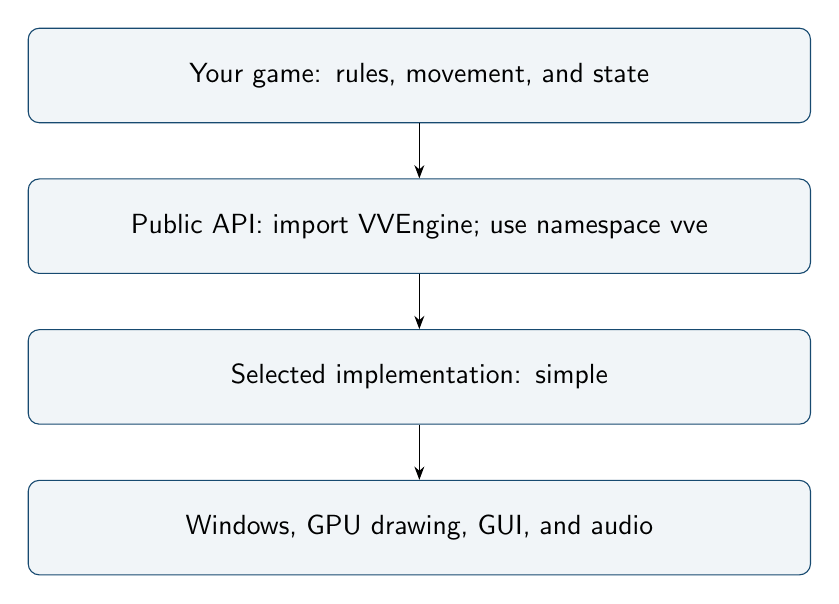
\begin{tikzpicture}[node distance=7mm,every node/.style={draw=vveblue,rounded corners,
    fill=vvelight,text width=0.8\linewidth,align=center,minimum height=12mm,font=\sffamily}]
    \node (game) {Your game: rules, movement, and state};
    \node (facade) [below=of game] {Public API: import VVEngine; use namespace vve};
    \node (engine) [below=of facade] {Selected implementation: simple};
    \node (gpu) [below=of engine] {Windows, GPU drawing, GUI, and audio};
    \draw[-{Stealth}] (game)--(facade);
    \draw[-{Stealth}] (facade)--(engine);
    \draw[-{Stealth}] (engine)--(gpu);
  \end{tikzpicture}\vfill
  {\normalsize Updated 16 October 2026\par}
  {\small Source baseline: 8f875a30; API checked against the local checkout.\par}
  {\small Game code uses the facade. Implementation chapters are for source study.\par}
  \end{titlepage}}
